\documentclass[addpoints]{exam}
\makeatletter
\expandafter\providecommand\expandafter*\csname ver@framed.sty\endcsname
{2003/07/21 v0.8a Simulated by exam}
\makeatother
\usepackage[top=1in, bottom=1in, left=1in, right=1in]{geometry}
\usepackage[utf8]{inputenc}
\usepackage[icelandic]{babel}
\usepackage[T1]{fontenc}
\usepackage[sc]{mathpazo}

\usepackage[parfill]{parskip}
\usepackage{booktabs,tabularx}
\usepackage{multirow}
\usepackage{multicol}
\usepackage{graphicx}
\usepackage{amsmath, amsfonts, amssymb, amsthm}
\usepackage{minted} %Minted and configuration
\usepackage{afterpage}
\usepackage{scrextend}

\usepackage[pdftex,bookmarks=true,colorlinks=true,pdfauthor={Eirikur Ernir Thorsteinsson},linkcolor=blue,urlcolor=blue]{hyperref}

\setcounter{secnumdepth}{-1} 
\hyphenpenalty=5000

\newcommand\blankpage{%
    \null
    \thispagestyle{empty}%
    \addtocounter{page}{-1}%
    \newpage}

\author{}
\date{}

\footer{}{}{}

\setcounter{secnumdepth}{-1} 

\qformat{\large \textbf Spurning \thequestion \phantom{M}(\totalpoints \phantom{l}stig) \hfill}
\renewcommand{\solutiontitle}{\noindent\textbf{Svar:}\par\noindent}
\renewcommand{\points}{stig}
\renewcommand{\questionshook}{\setlength{\itemsep}{0.5cm}}
\hqword{Spurning:}
\hpword{Stig í boði:}
\hsword{Stig:}
\htword{Samtals}

\title{TÖL105G Tölvunarfræði 1a - miðmisserispróf}
\author{}
\date{7. október 2017}

\pagestyle{headandfoot}
\firstpageheader{TÖL105G -\\ Tölvunarfræði 1a}{Miðmisserispróf}{7. október 2017\\12:00-13:30}
\firstpagefooter{}{Bls. \thepage\ af \numpages}{}
\runningfooter{}{Bls. \thepage\ af \numpages}{}
\setlength{\columnsep}{0.5cm}

% \printanswers
\begin{document}

% \thispagestyle{empty}
Fullt nafn: \vspace*{1mm} \hrule

\begin{center}
\begin{minipage}{.8\textwidth}
Á þessu prófi eru \numquestions\ spurningar sem samtals gefa 100 stig.
Ekki er dregið frá fyrir röng svör.
Skrifið svör í prófheftið.

Leyfileg hjálpargögn eru reiknivél og ein A4 blaðsíða af glósum.
\end{minipage}
\end{center}

\vspace{1cm}

\begin{questions}

\question Krossaspurningar. Merkið vandlega við réttan möguleika.

\begin{parts}
\part[5] Gefnar eru eftirfarandi Matlab-skipanir:
\begin{minted}{matlab}
>> a = (2 < 4) || (4 < 2);
>> b = (2 > 4) && (4 > 2);
\end{minted}
Hver verða gildi rökbreytanna $a$ og $b$ eftir að þær hafa verið keyrðar í skipanaglugganum?
\begin{checkboxes}
    \choice $a=0,b=0$
    \choice $a=0,b=1$
    \CorrectChoice $a=1,b=0$
    \choice $a=1,b=1$
    \choice Skipanirnar valda keyrsluvillu
\end{checkboxes}

\part[5] Hver af eftirfarandi Matlab-skipunum reiknar formúluna hér að neðan þegar \texttt{x} er skilgreint sem vigur (og \texttt{y} verður þá vigur líka)?
\[
    y = \left(\frac{4x}{x^3-\sin x^2}\right)^2
\]
\begin{checkboxes}
    \choice \verb|y = (4*x/(x^3 - sin(x^2)))^2|
    \choice \verb|y = (4*x/x^3 - sin(x^2))^2|
    \choice \verb|y = (4.*x/(x.^3 - sin(x.^2))).^2|
    \CorrectChoice \verb|y = (4*x./(x.^3 - sin(x.^2))).^2|
    \choice \verb|y = (4*x./(x.^3 - sin(x).^2)).^2|
\end{checkboxes}

\part[5] Hver eftirfarandi skipana skrifar út setninguna ``\texttt{Kvaðratrótin af 2 er um það bil 1.41}''?

\begin{checkboxes}
    \choice \verb|fprintf('Kvaðratrótin af 2 er um það bil%3.2f\n',sqrt(2))|
    \CorrectChoice \verb|fprintf('Kvaðratrótin af 2 er um það bil%5.2f\n',sqrt(2))|
    \choice \verb|fprintf('Kvaðratrótin af 2 er um það bil%4.2f\n',sqrt(2))|
    \choice \verb|fprintf('Kvaðratrótin af 2 er um það bil%4.2d\n',sqrt(2))|
    \choice \verb|fprintf('Kvaðratrótin af 2 er um það bil %f\n',sqrt(2))|
\end{checkboxes}

\vspace{1cm}
\begin{center}
    \gradetable[h][questions]
\end{center}

\part[5] Hvað skrifar eftirfarandi Matlab-forritsbútur út?

\begin{minted}[frame=lines]{matlab}
a = true;
b = true;
while a || b
    fprintf('%d%d', a, b);
    if a
        a = ~a;
    elseif ~a && b
        a = ~a;
        b = ~b;
    end
end
fprintf('%d%d\n', a, b);
\end{minted}

\begin{checkboxes}
    \choice \texttt{00}
    \choice \texttt{11}
    \choice \texttt{1101}
    \choice \texttt{11100100}
    \CorrectChoice \texttt{11011000}
\end{checkboxes}

\part[5] Gefið er eftirfarandi Matlab-fall:

\begin{minted}[frame=lines, label=f.m]{matlab}
function x = f(x)
x = x + 1;
y = x + 1;
end
\end{minted}
    
og eftirfarandi skipanir sem keyrðar eru í Matlab-skipanaglugganum:
    
\begin{minted}{matlab}
>> x = 1;
>> y = f(x)
\end{minted}
    
Hvert er gildi \texttt{y} í skipanaglugganum eftir að skipanirnar hafa verið keyrðar?
    
\begin{checkboxes}
    \choice \texttt{NaN}
    \choice 0
    \choice 1
    \CorrectChoice 2
    \choice 3
\end{checkboxes}

\part[5] Hver er stærsta heiltala sem hægt er að geyma í breytu af taginu \texttt{int32}?

\begin{checkboxes}
    \choice $32^2$
    \CorrectChoice $2^{31}-1$
    \choice $2^{31}+1$
    \choice $2^{32}-1$
    \choice $2^{32}$
\end{checkboxes}

\newpage
\part[5] Hvert er gildi breytunnar \texttt{t} eftir að eftirfarandi Matlab-skipanir hafa verið gefnar?

\begin{minted}{matlab}
>> x = 2;
>> x = x + 2;
>> t = num2str(x);
\end{minted}

\begin{checkboxes}
    \choice \texttt{NaN}
    \choice \texttt{'x'}, af taginu \texttt{char}
    \choice \texttt{'x'}, af taginu \texttt{double}
    \choice 4, af taginu \texttt{double}
    \CorrectChoice \texttt{'4'}, af taginu \texttt{char}
\end{checkboxes}

\end{parts}

\question Skrifið Matlab-skipanir (ein í hverjum lið) til að framkvæma eftirfarandi aðgerðir. Sé liðurinn leystur með meira en einni skipun fæst að hámarki eitt stig fyrir dæmið.
\begin{parts}
\part[3] Búið til $3 \times 4$ fylkið \texttt{a}, sem inniheldur jafndreifðar slembikommutölur á bilinu $]-2;2[$.
\vspace*{1.2cm}
\part[3] Eyðið út dálki 1 í \texttt{a}, svo að \texttt{a} verði að $3 \times 3$ fylki.
\vspace*{1.2cm}
\part[3] Breytið \texttt{a} í $4 \times 3$ fylki með því að bæta neðst í það línuvigrinum \verb|[1, 2, 3]|, sem yrði þá lína 4 í \texttt{a}.
\vspace*{1.2cm}
\part[3] Búið til breytuna \texttt{m}, sem inniheldur stærstu tölu í \texttt{a}. 
\vspace*{1.2cm}
\part[3] Vistið fylkið \texttt{a} í skrána \texttt{a.dat} á ascii-sniði.
\vspace*{1.2cm}
\end{parts}

\question Skrifið Matlab-skipanir (ein í hverjum lið) til að framkvæma eftirfarandi aðgerðir. Sé liðurinn leystur með meira en einni skipun fæst að hámarki eitt stig fyrir dæmið. 

Gefinn er vigur \texttt{v}, sem er ekki tómur. 
\begin{parts}
\part[3] Sýnið eina Matlab-skipun sem breytir \texttt{v} svo hann innihaldi eingöngu þau gildi sem voru í oddatölusætum.
\vspace*{1.2cm}
\part[3] Búið til rökbreytuna \texttt{r}, sem inniheldur 1 ef öll stök stök \texttt{v} hafa sama gildið, annars 0.
\end{parts}

\begin{solution}

\begin{minted}{matlab}
>> v = v(1:2:end);
>> r = all(v == v(1));
\end{minted}

\end{solution}

\newpage
\question[4] Sýnið Matlab-skipanir sem teikna fallið $e^{-0.5x}\sin(x)$ á bilinu $[0;10]$. Hafið teikninguna rauða á litinn með stjörnu í gagnapunktum. Gagnapunktarnir skulu vera um 100 talsins.
Útkoman væri þá nokkuð lík eftirfarandi mynd:
\begin{center}
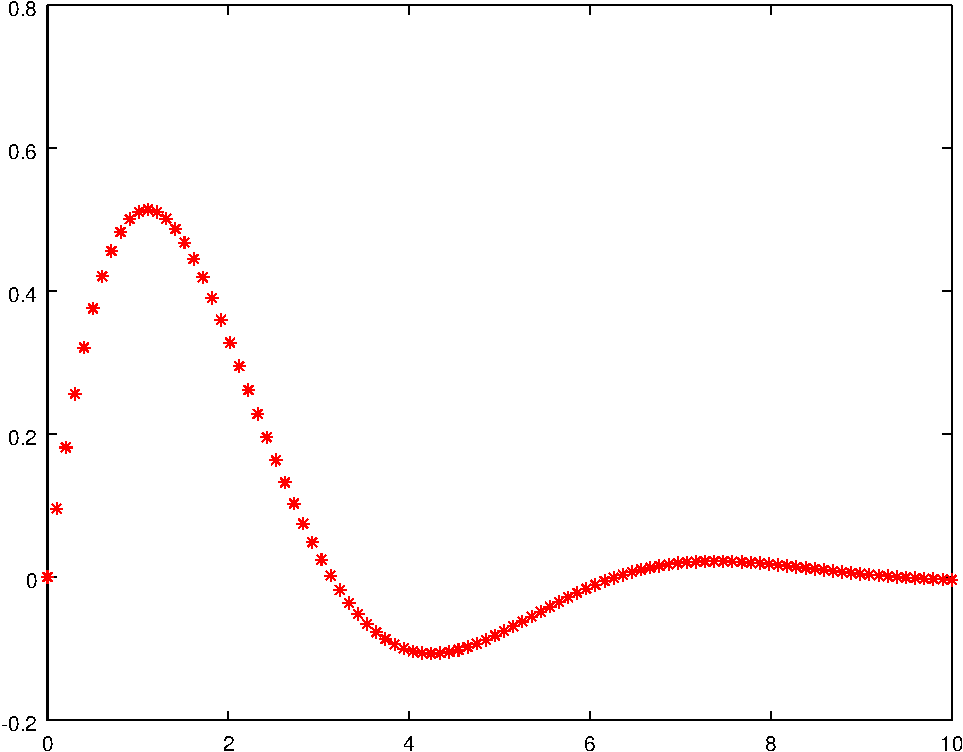
\includegraphics[width=0.5\textwidth]{Pics/expsin}
\end{center}

\vspace{5cm}

\begin{solution}
 
\begin{minted}{matlab}
>> x = linspace(0,10);
>> y = exp(-0.5*x).*sin(x);
>> plot(x, y, 'r*')
\end{minted}

\end{solution}

\newpage
\question[10] Skrifið Matlab-skipanaskrá sem biður notanda um að slá inn hliðarlengd og skrifar út ferning af stjörnum og myllumerkjum á eftirfarandi sniði (þar sem stærðin er í samræmi við inntakið):
\begin{minted}{matlab}
>> starsquare % Hér heitir forritið "starsquare"
Hversu stór á ferningurinn að vera? 5
*####
**###
***##
****#
*****    
\end{minted}

\begin{solution}
\begin{minted}{matlab}
n = input('Hversu stór á ferningurinn að vera? ');

for i = 1:n
    for j = 1:n
        if i >= j
            fprintf('*')
        else
            fprintf('#')
        end
    end
    fprintf('\n')
end
\end{minted}
\end{solution}

\newpage
\question[10] Eftirfarandi röð, þar sem jákvæðir og neikvæðir liðir skiptast á og nefnari liðsins hækkar um 2 með hverjum lið,  \[y = 1 - \frac{1}{3} + \frac{1}{5} - \frac{1}{7} + \frac{1}{9}- \ldots\] nálgast töluna $\frac{\pi}{4}$ meir og meir eftir því sem liðunum fjölgar.

Skrifið Matlab-forrit sem reiknar summu liða raðarinnar þar til mismunurinn á þeirri summu og einum fjórða af innbyggða gildinu á $\pi$ er minni en eða jafn $10^{-5}$ og skrifar út hversu marga liði þurfti.

Dæmi um mögulega keyrslu forritsins:

\begin{minted}{matlab}
>> pisum % Hér er forritið í pisum.m
25000 liði þurfti.
\end{minted}

\begin{solution}

\begin{minted}[frame=lines]{matlab}
y = 0;
i = 0;
while abs(pi/4 - y) > 1e-4
    y = y + (-1)^i/(i*2+1);
    i = i + 1;
end
disp([num2str(i) ' liði þurfti.'])
\end{minted}

\end{solution}

\newpage
\question[10] Hamming-fjarlægð er einfaldur mælikvarði á hversu ólíkir tveir jafn langir strengir eru. Hún er skilgreind sem fjöldi þeirra sæta þar sem strengirnir innihalda ekki sömu tákn.

Skrifið Matlab-fallið \texttt{hammingdistance}, sem reiknar út Hamming-fjarlægð. Fallið skal gefa villu sé reynt að nota það á strengi sem ekki eru jafn langir.

Dæmi um mögulega keyrslu fallsins:
\begin{minted}{matlab}
>> hammingdistance('Nonni','Jonni')
ans =
      1
>> hammingdistance('Nommi','Jonni')
ans =
      3
>> hammingdistance('Sjonni','Jonni') % Veldur villu
\end{minted}


\begin{solution}
 
\begin{minted}{matlab}
function d = hammingdistance(s1,s2)
  d = sum(s1~=s2);
end
\end{minted}

\end{solution}

\newpage

\question[10] Skrifið Matlab-fallið \texttt{trianglearea} sem tekur inn tvo þriggja staka talnavigra, þar sem fyrri vigurinn táknar $x$-hnit þríhyrnings og seinni vigurinn táknar $y$-hnit hans. Fallið skal skila flatarmáli þríhyrningsins.

Hægt er að reikna fjarlægð á milli punktanna $(x_1,y_1)$ og $(x_2,y_2)$ með eftirfarandi formúlu:
\[
    d = \sqrt{(x_2-x_1)^2 + (y_2-y_1)^2}
\]
Hægt er að reikna flatarmál þríhyrnings með hliðarlengdir $a,b$ og $c$ með reglu Herons:
\[
    A = \sqrt{s(s-a)(s-b)(s-c)}
\]
með $s=\frac{a+b+c}{2}$.

Dæmi um mögulega keyrslu fallsins:
\begin{minted}{matlab}
>> x = [0 1 0]; y = [0 0 1]; % Þríhyrningur sem fyllir upp í hálfan einingaferninginn
>> trianglearea(x,y)
ans =
    0.5000
\end{minted}

\begin{solution}
\begin{minted}{matlab}
function area = trianglearea(x,y)
a = distance(x(1),x(2),y(1),y(2));
b = distance(x(2),x(3),y(2),y(3));
c = distance(x(3),x(1),y(3),y(1));
area = heron(a,b,c);
end

function d = distance(x1,x2,y1,y2)
d = sqrt((x2-x1).^2 + (y2-y1).^2);
end

function area = heron(a,b,c)
s = (a+b+c)/2;
area = sqrt(s*(s-a)*(s-b)*(s-c));
end
\end{minted}
\end{solution}

\end{questions}
\end{document}
